\documentclass[sigplan]{acmart}
\usepackage{graphicx}

\AtBeginDocument{%
  \providecommand\BibTeX{{%
    \normalfont B\kern-0.5em{\scshape i\kern-0.25em b}\kern-0.8em\TeX}}}

\setcopyright{rightsretained}
\copyrightyear{2023}

%% Following attributes are not applicable to this report
%% Left blank in a manner which is minimally invasive to the reading experience

\acmYear{}
\acmDOI{}

\acmConference[]{}{}{}

\acmBooktitle{} 
\acmPrice{}
\acmISBN{}

\settopmatter{printacmref=false}

\begin{document}

\title{A Report on Experimentations With Machine Learning Models}

\author{Charles Hu}
\email{czhu06@wm.edu}
\affiliation{%
  \institution{College of William \& Mary}
  \city{Williamsburg}
  \state{Virginia}
  \country{USA}
}

\maketitle

\section{Introduction}

The following is a report on the experimental findings of reproducing and adapting the model architectures used for convolutional neural networks, transformers, and autoencoders as based on the notable papers which introduced such architectures. The produced models used for this report are all written using the TensorFlow framework using the Keras API and attempt to replicate the originally presented architectures and preserve their logical structures as faithfully as possible with little to no disruptive alterations unless necessary. What follows is an outline and inspection of the results of these produced models.

\section{Convolutional neural networks for image analysis}

Image analysis was performed using deep learning residual networks and the CIFAR-10 image data set as described in He et al. [2015]. In particular, the ResNet50 and ResNet101 model architectures were trained and tested on the CIFAR-10 data set provided by the Keras API.

The implemented ResNet50 and ResNet101 models used the ResNet50 and ResNet101 architecture presets provided by Keras with adjustments made to the input and output layers to better facilitate the CIFAR-10 data set. These alterations followed the architectural design described in the paper. The input layer was composed of a 32x32x3 (the default size of the CIFAR-10 images) network input layer and the output layer was composed of a global average pooling layer, a 10-class (the amount of classes available in CIFAR-10) fully connected layer, and a softmax activation function. Models were trained over 10 epochs as opposed to the 10k used in the paper due to resource constraints.

The CIFAR-10 data set was split into 45k training images, 5k validation images, and 10k testing images. All images were preprocessed to convert the color channel format from RGB to BGR and zero-center the color channel with respect to the ImageNet data set. The only deviation from the paper was the use of a 10-crop image augmentation function on the validation and testing sets to produce a 10-crop version of each set which was only used for the ImageNet data set in the original paper.

\begin{figure}[h]
  \centering
  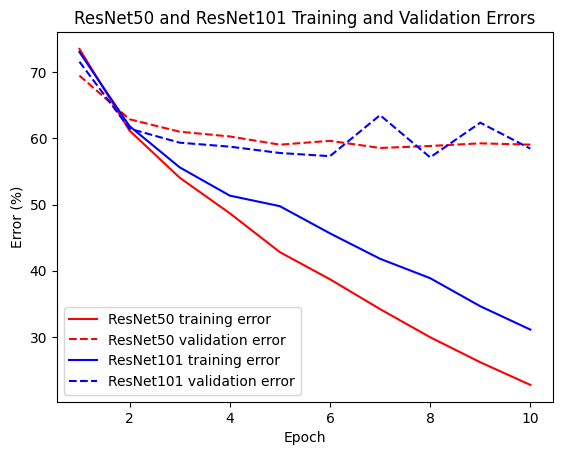
\includegraphics[width=\linewidth]{resnetErr.png}
  \caption{Training and validation errors across the ResNet50 and ResNet101 models.}
  \Description{A graph showing training and validation error rates across both the ResNet50 and ResNet101 models.}
\end{figure}

Both error rates for training and validation decreased as expected during model training (see Fig. 1). Throughout the process, ResNet50 maintained lower error than ResNet101 for training but ResNet101 appeared to outperform ResNet50 for validation error during most of the epochs. Additionally a large gap between training and validation error began to appear as epoch count increased.

Interestingly, in Fig. 4 in He et al. [2015] we observe a surprisingly different trend for early epochs where validation error is lower than training error consistently until 300k epochs. Conversely, the order of the models seem to mirror somewhat with lower layered models (i.e., ResNet50 here and ResNet18 there) initially beating out higher layered models until around 50k epochs, which one could potentially reason as per all layers finally being utilized for higher layered models after a large amount of training epochs. Of course, direct comparison is difficult as both the used models and epoch count are not equal, however, Fig. 4 in He et al. [2015] may potentially allude to possible trends or design differences for our current models given greater epoch counts.

If, during future work involving greater epochs counts, our current models begin to mirror the results shown in the other paper's Fig. 4, it may allow some better establishment of a correlation between ResNet layer size, error rates, and epoch counts. If the opposite were true, then it may allude to some difference in architectural or procedural design or potentially even an error in either models.

Model testing involved re-creating Table 3 and Table 4 from He et al. [2015] using the CIFAR-10 validation set, testing set, and a 10-crop version of the validation and testing set (see Table 1 and Table 2). Unlike the source paper, the model testing here included the testing set to provide a better out of sample generalization measure.

The model tests revealed consistently high top-1 error across both 10-crop and standard testing, but the tests also produced generally acceptable top-5 error. This seems to indicate that while the models struggled to predict the correct class for a given image, they were able to associate the correct class for the image within their top 5 class predictions. Of course, increased epoch count in future work may be able to decrease the magnitude of these error rates, but the general pattern observed here should still hold.

Additionally, error rates for a given error category (i.e., top-1 or top-5 error) were surprisingly similar across both model types for each testing procedure. This does seem to correlate with Tables 3 and 4 in He et al. [2015], which show similar behavior for ResNet50 and ResNet101 models across their top-5 and top-1 error categories. This may suggest some level of diminishing returns for deeper and deeper learning models compared to gains observed between shallow and deep learning models.

\begin{table}
  \caption{Error rates (\%, 10-crop testing) on CIFAR-10 validation and testing sets. Top half shows validation set rates, bottom half shows testing set rates.}
  \label{tab:err10}
  \begin{tabular}{ccc}
    \toprule
    Model & Top-1 err. & Top-5 err. \\
    \midrule
    ResNet50 & 73.27 & 22.80 \\
    ResNet101 & 73.72 & 23.73 \\
    \midrule
    ResNet50 & 73.27 & 22.37 \\
    ResNet101 & 73.37 & 23.47 \\
    \bottomrule
  \end{tabular}
\end{table}

\begin{table}
  \caption{Error rates (\%) of single-model results on the CIFAR-10 validation and testing sets. Top half shows validation set rates, bottom half shows testing set rates.}
  \label{tab:errStd}
  \begin{tabular}{ccc}
    \toprule
    Method & Top-1 err. & Top-5 err. \\
    \midrule
    ResNet50 & 59.06 & 12.20 \\
    ResNet101 & 58.46 & 11.94 \\
    \midrule
    ResNet50 & 57.99 & 10.86 \\
    ResNet101 & 56.82 & 11.13 \\
    \bottomrule
  \end{tabular}
\end{table}

\section{Transformers for text analysis}

Image analysis was performed using source code from a prebuilt transformer model [5] with the addition of custom testing code to provide model testing for the transformer on the Keras-provided IMDB movie review sentiment data set.

Testing involved the random sampling of 100 user review text bodies from the IMDB test set, where each review is encoded as a list of word indices ordered by overall word frequency. The sample was then preprocessed to limit each word list to the top 200 most frequently occurring words (which was similarly performed on the training set during model training). The model was then given a classification task where it had to predict the movie review rating for each given review in the sample. A prediction of class 0 corresponded to a negative review and a prediction of class 1 corresponded to a positive review.

\begin{figure}[h]
  \centering
  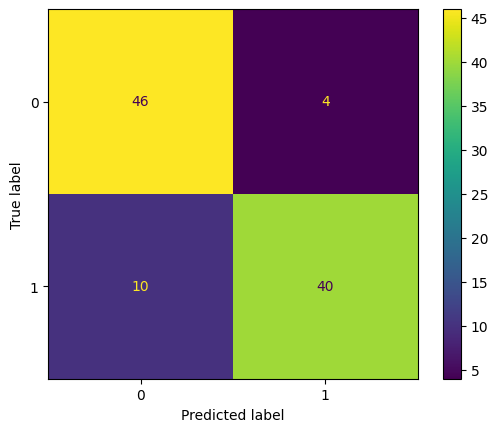
\includegraphics[width=\linewidth]{confusion.png}
  \caption{Confusion matrix tracking model sentiment classifications for sample movie reviews. Class 0 corresponds to a negative review while class 1 corresponds to a positive review.}
  \Description{A confusion matrix tracking correct and incorrect sentiment classifications for movie reviews.}
\end{figure}

Fig. 2 shows the results of the classification task. The model achieved 86\% accuracy on the sampled test set. In cases where the model incorrectly classified the review's class, the model was more likely to misclassify a positive review as a negative review as opposed to the opposite scenario. This may potentially arise due to these positive reviews containing certain criticisms which include phrases or key words the model has learned to associate with negative reviews. An inclusion of more mixed content reviews (i.e., positive reviews containing criticisms or negative reviews containing praises) could possible temper this effect in the model and improve classification accuracy on this front.

Testing of this model outside of the data set that was used to train it was difficult within the confines of the available natural language sets on Keras due to the nature of how these data sets were designed. As words are indexed via overall frequency in the IMDB data set, the model is inherently tied to this specific data set, making generalizability poor for other data sets which do not adopt the same index mapping for words. Future work expanding on this model and its generalizability necessitates either creating a system which translates other data sets to the IMDB data set index mapping or adopting a more universally accepted word mapping methodology and training the model over that.

\section{Variational autoencoder for image analysis}

Image analysis was performed using a variational autoencoder and the MNIST digits data set, which were sourced from a code implementation originally designed using the PyTorch framework [1] and migrated over to the TensorFlow and Keras framework for the purposes of this experiment. Model training was broken down into 2 different experiments in which both the model optimizer and the 0.5 coefficient in the KL divergence expression in the loss function were parameterized and varied.

The baseline for the optimizer experiment was the Adam optimizer, which was the default optimization method used in both the PyTorch and TensorFlow implementations. Over 10 epochs and with a learning rate of 1e-3, the optimizer obtained a final average loss of 107.9837 and a final test set loss of 96.3758. Using the same epoch count and learning rate, 5 different optimizers were tested against this baseline: Adadelta, Adamax, Ftrl, Lion, and the RMSprop optimizer.

Of these optimizers, Adadelta and Ftrl failed to make any improvements over the baseline. Adadelta's poor performance compared to Adam is expected as Adam uses the same mechanics as Adadelta but also utilizes momentum to optimize gradients. For Ftrl, this could be due to the optimizer's original design for shallow models with a large and sparse feature space making it incompatible with the current model specifications.

Adamax had marginal gains with a final average loss of 100.9554 and final test set loss of 92.6330. Similar to Adadelta and Adam, Adamax is an extension of Adam which performs an optimization to the Adam update rule, explaining our observed results. Lion showed rather substantial gains with a final average loss of 92.5047 and final test set loss of 85.8458. Purportedly, improvements over Adam are due to its use of a sign operation which improves model generalizability [2]. RMSprop also made impressive gains over Adam with a final average loss of 95.4400 and final test set loss of 86.8105. This is the most interesting result as RMSprop is one of the few optimizers tested here that does not incorporate momentum as a mechanic. While the results shown here do not explicitly allude to any clear reason as to why RMSprop outperforms some of its momentum-based counterparts, it could warrant further investigation as to what specifically (e.g., learning rate, epoch count, model specifications) evokes this result.

The KL divergence coefficient parameterization experiment involved the generation of new models over a coefficient range of 0.1 to 5.0 inclusive with iterative steps of 0.1 and observing the final average loss and final test set loss over 10 epochs. The results of these models were then compared to a baseline model using a coefficient of 0.5 with 107.9837 final average loss and 96.3758 final test set loss.

Experimental results over this range suggest a positive correlation between the coefficient value and the magnitude of the final average loss and final test set loss. A coefficient value of 0.1 achieved 77.5693 final average loss and 74.3500 final test set loss while a coefficient value of 0.5 achieved 160.7043 final average loss and 139.5759 final test set loss, which was much higher than the baseline.

This possibly suggests that a lower coefficient term results in greater regularization and thus better generalizability for this specific VAE model scenario. Applicability of these results outside of this use case are still unknown, and potential future work could involve expanding this experimental scenario across different data sets and longer training iterations to reaffirm the results derived from this experiment.

\bibliographystyle{ACM-Reference-Format}
\nocite{*}
\bibliography{citation}

\end{document}
